% Case-C comparison of the translational stiffness along t_2. The legend gives the
% achieved pose-based initial angular-offset range across the three settings.
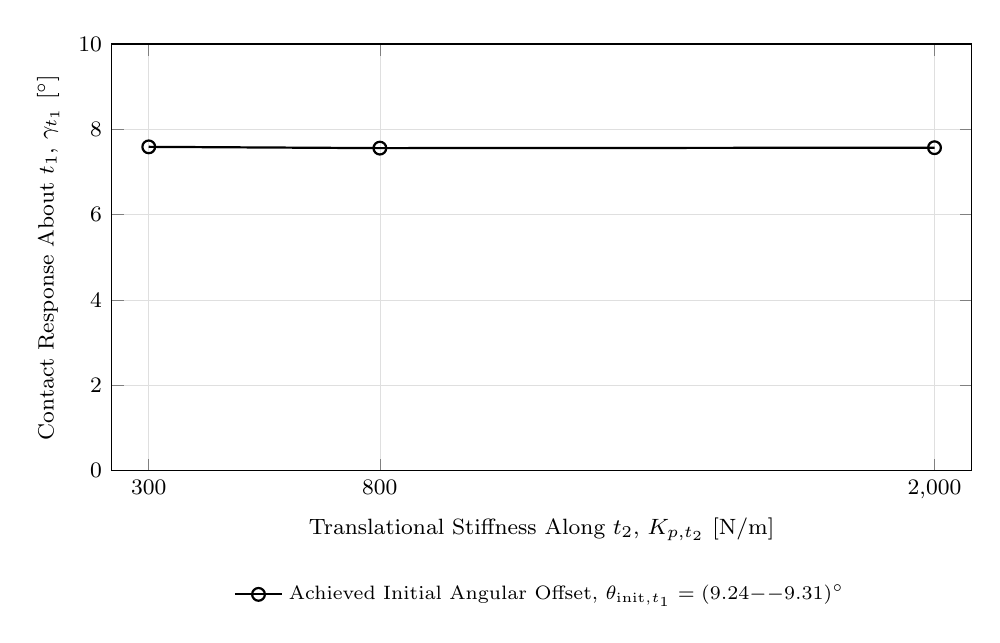
\begin{tikzpicture}
\begin{axis}[
    width=12.5cm, height=7.0cm,
    xmin=220, xmax=2080, ymin=0, ymax=10,
    xtick={300,800,2000},
    ytick={0,2,4,6,8,10},
    grid=major,
    grid style={gray!25, very thin},
    tick label style={font=\footnotesize},
    label style={font=\footnotesize},
    xlabel={Translational Stiffness Along \(t_2\), \(K_{p,t_2}\) [N/m]},
    ylabel={Contact Response About \(t_1\), \(\gamma_{t_1}\) [\(^\circ\)]},
    legend style={font=\scriptsize, draw=none, fill=none,
                  cells={anchor=west}, at={(0.5,-0.24)}, anchor=north},
    every axis plot/.append style={thick, mark size=2.3pt},
  ]
\addplot[black, mark=o] coordinates {
  (300,7.59) (800,7.56) (2000,7.57)};
\addlegendentry{Achieved Initial Angular Offset, \(\theta_{\mathrm{init},t_1}=(9.24\text{--}9.31)^\circ\)}
\end{axis}
\end{tikzpicture}
